\section{Rozwiązanie problemu} 

\begin{frame}
    \frametitle{Integracja modeli symulacyjnych}
    \begin{figure}
        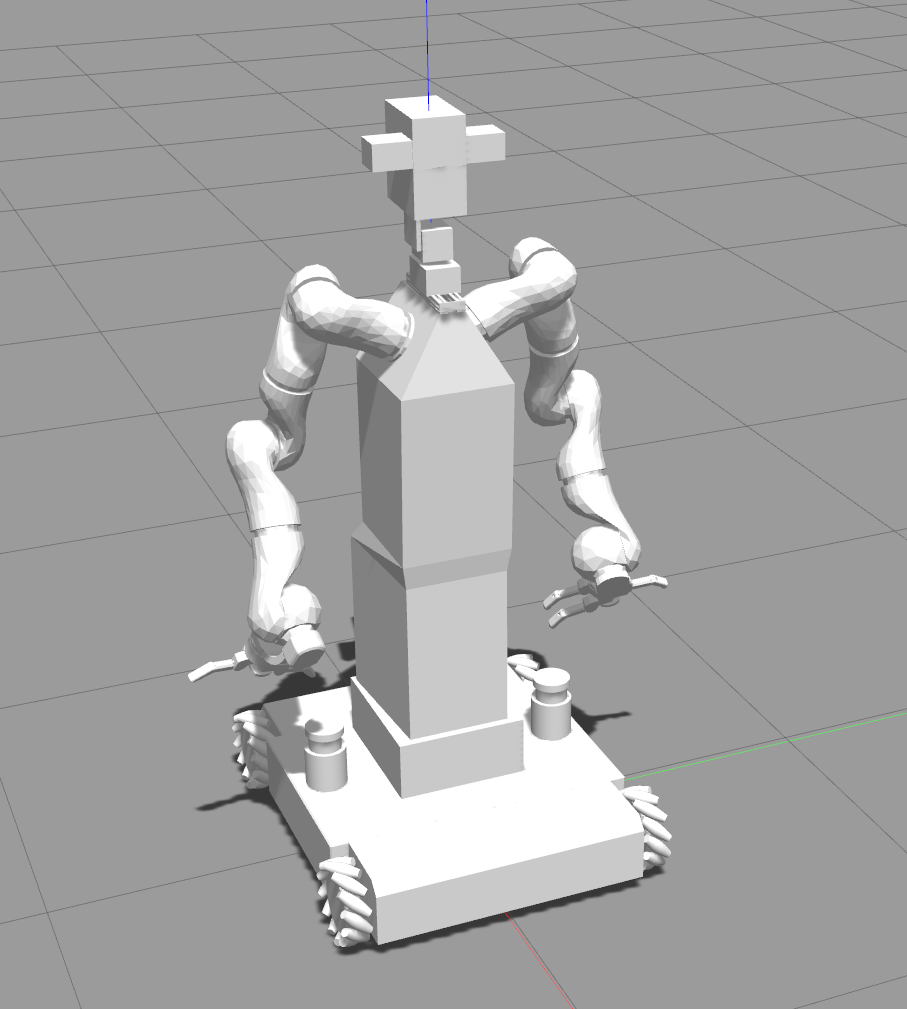
\includegraphics[scale=0.20]{./images/omnivelmobil-final-cropped.png}
        \caption{Zintegrowany robot Velma w symulatorze Gazebo}
    \end{figure}
\end{frame}

\begin{frame}
    \frametitle{Ogólna struktura projektowanego systemu} 
    \begin{figure}[b]
        \label{system_overview}
        \centering
        \def\svgwidth{\columnwidth}
        \vspace{0.1cm}
        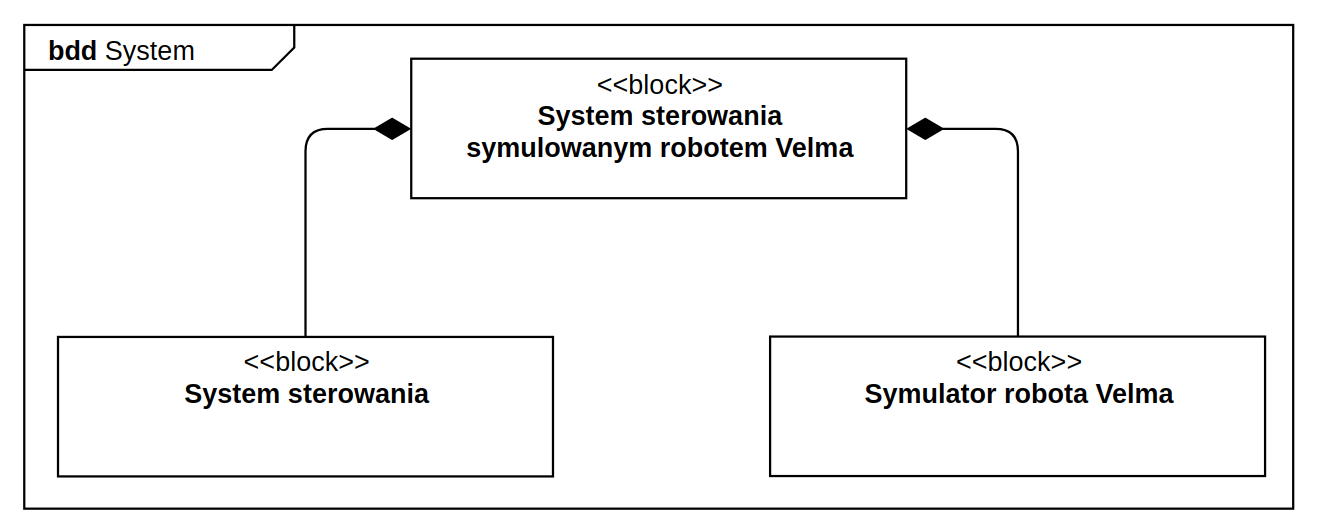
\includegraphics[scale=0.25]{images/basic_system.png}
        \vspace{0.1cm}
        \caption{Bazowa struktura projektowanego systemu}
    \end{figure}
\end{frame}

\begin{frame}
    \frametitle{Struktura symulatora robota Velma} 
    \begin{figure}[b]
        \label{sim_system}
        \centering
        \def\svgwidth{\columnwidth}
        \vspace{0.1cm}
        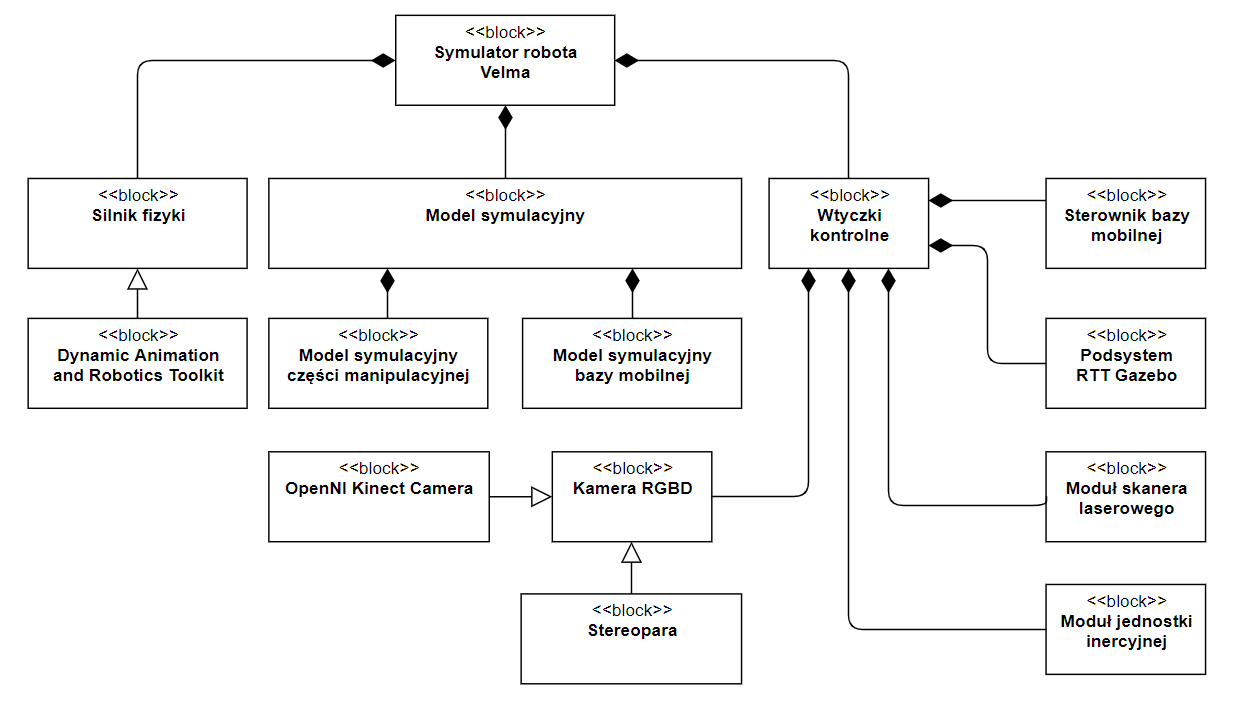
\includegraphics[scale=0.35]{images/sim_system.png}
        \vspace{0.1cm}
        \caption{Struktura symulatora robota Velma}
    \end{figure}
\end{frame}

\begin{frame}
    \frametitle{Zasada działania sterownika bazy mobilnej} 
    \begin{block}{Sterownik bazy mobilnej}
        Baza mobilna traktowana jest jak prostopadłościan przesuwany za pomocą prostopadle przyłożonych
        sił w osi $OX$ oraz $OY$ oraz obracany momentem siły w osi $OZ$.
    \end{block}

    \begin{block}{Interfejs}
        Z nowym sterownikiem komunikacja zachodzi poprzez ujednolicony interfejs prędkościowy.
        Komponent odczytuje prędkość zadaną z tematu \texttt{/cmd\_{}vel}
    \end{block}
\end{frame}

\begin{frame}
    \frametitle{Struktura systemu sterowania} 
    \begin{figure}[b]
        \label{control_system}
        \centering
        \def\svgwidth{\columnwidth}
        \vspace{0.1cm}
        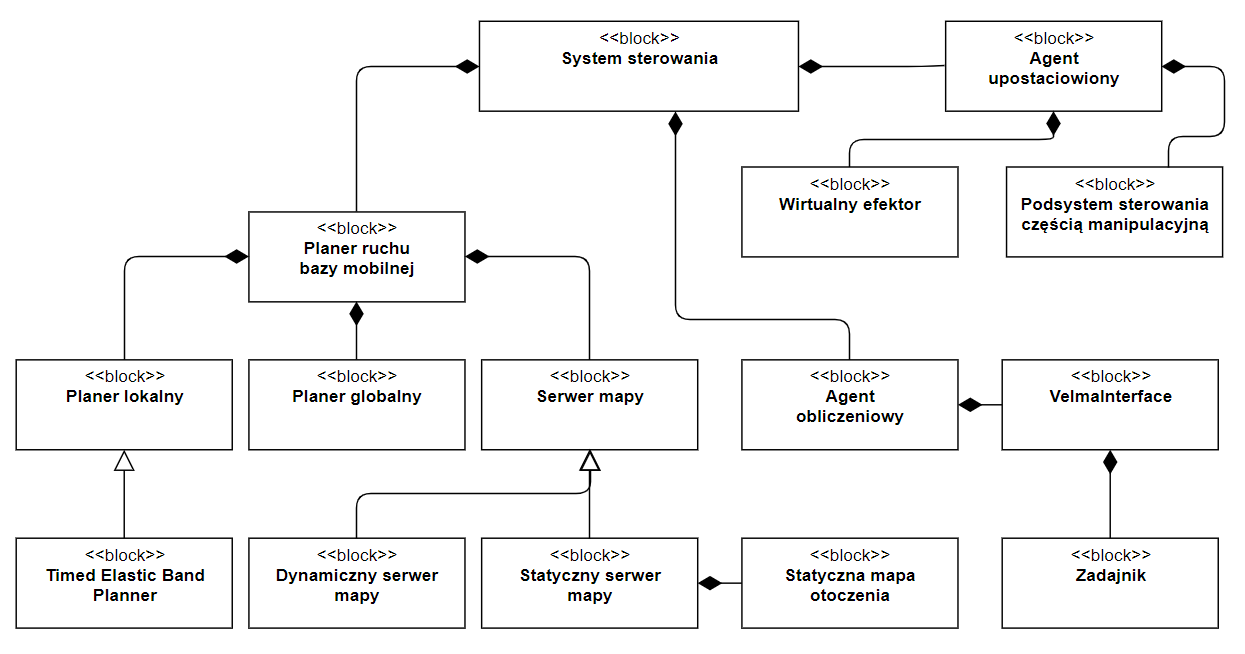
\includegraphics[scale=0.35]{images/control_system.png}
        \vspace{0.1cm}
        \caption{Struktura sterowania robotem Velma}
    \end{figure}
\end{frame}




